\documentclass[14pt]{extarticle}
\usepackage[landscape, margin=0.5in]{geometry}
\usepackage{lipsum}
\usepackage[T1]{fontenc}
\usepackage{tgheros}
\setlength{\emergencystretch}{3em} % prevent overfull lines
\providecommand{\tightlist}{%
  \setlength{\itemsep}{0pt}\setlength{\parskip}{0pt}}
\usepackage{textcomp} % provide euro and other symbols
\usepackage{xcolor}

\definecolor{gemgreen}{HTML}{98C9AF}
\definecolor{gemblue}{HTML}{8EAACC}
\usepackage{multicol}
\setlength{\columnsep}{0.5in}

\usepackage{amsmath,amssymb}
\usepackage{iftex}
\ifPDFTeX
  \usepackage[T1]{fontenc}
  \usepackage[utf8]{inputenc}
  \usepackage{textcomp} % provide euro and other symbols
\else % if luatex or xetex
  \usepackage{unicode-math} % this also loads fontspec
  \defaultfontfeatures{Scale=MatchLowercase}
  \defaultfontfeatures[\rmfamily]{Ligatures=TeX,Scale=1}
\fi
\usepackage{lmodern}
\ifPDFTeX\else
  % xetex/luatex font selection
\fi
% Use upquote if available, for straight quotes in verbatim environments
\IfFileExists{upquote.sty}{\usepackage{upquote}}{}
\IfFileExists{microtype.sty}{% use microtype if available
  \usepackage[]{microtype}
  \UseMicrotypeSet[protrusion]{basicmath} % disable protrusion for tt fonts
}{}
\makeatletter
\@ifundefined{KOMAClassName}{% if non-KOMA class
  \IfFileExists{parskip.sty}{%
    \usepackage{parskip}
  }{% else
    \setlength{\parindent}{0pt}
    \setlength{\parskip}{6pt plus 2pt minus 1pt}}
}{% if KOMA class
  \KOMAoptions{parskip=half}}
\makeatother
\usepackage{xcolor}
\usepackage{longtable,booktabs,array}
\usepackage{calc} % for calculating minipage widths
% Correct order of tables after \paragraph or \subparagraph
\usepackage{etoolbox}
\makeatletter
\patchcmd\longtable{\par}{\if@noskipsec\mbox{}\fi\par}{}{}
\makeatother
% Allow footnotes in longtable head/foot
\IfFileExists{footnotehyper.sty}{\usepackage{footnotehyper}}{\usepackage{footnote}}
\makesavenoteenv{longtable}
\usepackage{graphicx}
\makeatletter
\def\maxwidth{\ifdim\Gin@nat@width>\linewidth\linewidth\else\Gin@nat@width\fi}
\def\maxheight{\ifdim\Gin@nat@height>\textheight\textheight\else\Gin@nat@height\fi}
\makeatother
% Scale images if necessary, so that they will not overflow the page
% margins by default, and it is still possible to overwrite the defaults
% using explicit options in \includegraphics[width, height, ...]{}
\setkeys{Gin}{width=\maxwidth,height=\maxheight,keepaspectratio}
% Set default figure placement to htbp
\makeatletter
\def\fps@figure{htbp}
\makeatother
\setlength{\emergencystretch}{3em} % prevent overfull lines
\providecommand{\tightlist}{%
  \setlength{\itemsep}{0pt}\setlength{\parskip}{0pt}}
\setcounter{secnumdepth}{-\maxdimen} % remove section numbering
% Make \paragraph and \subparagraph free-standing
\ifx\paragraph\undefined\else
  \let\oldparagraph\paragraph
  \renewcommand{\paragraph}[1]{\oldparagraph{#1}\mbox{}}
\fi
\ifx\subparagraph\undefined\else
  \let\oldsubparagraph\subparagraph
  \renewcommand{\subparagraph}[1]{\oldsubparagraph{#1}\mbox{}}
\fi
\makeatletter
\makeatother
\makeatletter
\makeatother
\makeatletter
\@ifpackageloaded{caption}{}{\usepackage{caption}}
\AtBeginDocument{%
\ifdefined\contentsname
  \renewcommand*\contentsname{Table of contents}
\else
  \newcommand\contentsname{Table of contents}
\fi
\ifdefined\listfigurename
  \renewcommand*\listfigurename{List of Figures}
\else
  \newcommand\listfigurename{List of Figures}
\fi
\ifdefined\listtablename
  \renewcommand*\listtablename{List of Tables}
\else
  \newcommand\listtablename{List of Tables}
\fi
\ifdefined\figurename
  \renewcommand*\figurename{Figure}
\else
  \newcommand\figurename{Figure}
\fi
\ifdefined\tablename
  \renewcommand*\tablename{Table}
\else
  \newcommand\tablename{Table}
\fi
}
\@ifpackageloaded{float}{}{\usepackage{float}}
\floatstyle{ruled}
\@ifundefined{c@chapter}{\newfloat{codelisting}{h}{lop}}{\newfloat{codelisting}{h}{lop}[chapter]}
\floatname{codelisting}{Listing}
\newcommand*\listoflistings{\listof{codelisting}{List of Listings}}
\makeatother
\makeatletter
\@ifpackageloaded{caption}{}{\usepackage{caption}}
\@ifpackageloaded{subcaption}{}{\usepackage{subcaption}}
\makeatother
\makeatletter
\@ifpackageloaded{tcolorbox}{}{\usepackage[skins,breakable]{tcolorbox}}
\makeatother
\makeatletter
\@ifundefined{shadecolor}{\definecolor{shadecolor}{rgb}{.97, .97, .97}}
\makeatother
\makeatletter
\makeatother
\makeatletter
\makeatother
\ifLuaTeX
  \usepackage{selnolig}  % disable illegal ligatures
\fi
\IfFileExists{bookmark.sty}{\usepackage{bookmark}}{\usepackage{hyperref}}
\IfFileExists{xurl.sty}{\usepackage{xurl}}{} % add URL line breaks if available
\urlstyle{same}
\hypersetup{
  colorlinks=true,
  linkcolor={blue},
  filecolor={Maroon},
  citecolor={Blue},
  urlcolor={Blue},
  pdfcreator={LaTeX via pandoc}}

\author{}
\date{}

\usepackage{wrapfig}
\begin{document}

\pagecolor{gemgreen}
\begin{multicols}{3}


\ifdefined\Shaded\renewenvironment{Shaded}{\begin{tcolorbox}[enhanced, breakable, frame hidden, sharp corners, interior hidden, boxrule=0pt, borderline west={3pt}{0pt}{shadecolor}]}{\end{tcolorbox}}\fi

\thispagestyle{empty}
\hrule

\textbf{Join us at the next GemCity TECH event to:}

\begin{itemize}
\tightlist
\item
  Deepen your knowledge in a:

  \begin{itemize}
  \tightlist
  \item
    technology or
  \item
    discipline
  \end{itemize}
\item
  Grow your skills
\item
  Diversify your skills or get your feet wet in a topic of interest
\item
  Expand your network of technology professionals
\item
  Find like minded people to collaborate on your project
\item
  Share your knowledge by speaking it at an event
\item
  Talk to GemCity TECH leaders about starting your own community in the
  GemCity TECH family
\item
  Help grow local industry by:

  \begin{itemize}
  \tightlist
  \item
    sponsoring
  \item
    attending
  \end{itemize}
\end{itemize}

\hfill

\hrule

\makebox[3.1in][c]{
  
\includegraphics[width=1.1in]{./img/GemCity_meetup_qr.png}}

\makebox[3.1in][c]{\textbf{GemCity.TECH}}

\columnbreak

\textbf{Our Groups}\\
Each of our monthly user groups brings people together to explore and
learn about technology. We provide a platform for people to get
involved, exercise new skills make new friends and build a support
system. There are multiple opportunities to share your knowledge, learn
from others and take ownership of your own community.

\textbf{Where do we meet?}\\
Arcade's Innovation Hub

Our partner, the \textbf{Arcade’s Innovation Hub}, offers a variety of
meeting spaces for our groups. The Arcade is a historic complex located
in Dayton's central business district. It features elegant architecture
with grand and open spaces.

We'll gladly give you a tour of the beautiful collaboration space.

Contact us on our Discord Server

\makebox[3.15in][c]{
  
\includegraphics[width=1.1in]{img/gemcity_discord_qr.png}}

\columnbreak


\includegraphics{img/GCTSquareWhiteForeground.png}

\textbf{Dayton's Tech Community}

GemCity TECH provides a centralized destination for technical training,
workshops, forums and opportunities to collaborate in the Dayton, Ohio
area.

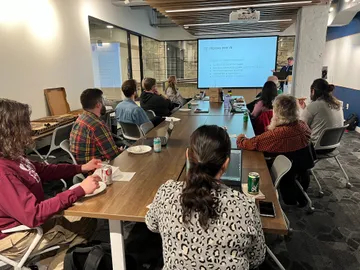
\includegraphics{img/meetup_image.jpg}

\hrule

\hrule

\makebox[3.1in][c]{
  
\includegraphics[width=1.1in]{./img/GemCity_meetup_qr.png}}

\makebox[3.1in][c]{\textbf{GemCity.TECH}}



\end{multicols}
\end{document}
